% ABLS - term-long paper

\documentclass{sig-alternate}

\usepackage{url}
\usepackage{color}
\usepackage{enumerate}
\usepackage{balance}
\usepackage{verbatim}
\usepackage{enumitem}
\usepackage[table]{xcolor}
\usepackage{multicol,multirow}
\usepackage{subfig}
\usepackage{dcolumn}
\usepackage{palatino}
\usepackage{bbm}
\usepackage{url}
\usepackage{verbatim}
\usepackage{algorithm}
\usepackage[noend]{algorithmic}
\usepackage{fancybox, fancyvrb}
\usepackage{listings}
\usepackage{amsmath}
\usepackage{array}
\usepackage{txfonts}

\permission{}
\CopyrightYear{2012}
%\crdata{0-00000-00-0/00/00}
\begin{document}

\title{ABLS - An Attribute Based Logging System for the Cloud}
\numberofauthors{1}
\author{
\alignauthor{
Christopher A. Wood \\
Department of Computer Science \\
{\tt caw4567@rit.edu}
}}
\date{\today}
\maketitle
\begin{abstract}
User-based non-repudiation is an increasingly important property of cloud-based applications. It provides irrefutable evidence that ties system behavior to specific users, which in turn enables the strict enforcement of organizational security policies. System logs, which can be used to construct audit trails, are typically used as the basis for this property. Thus, the effectiveness of system audits based on log files reduces to the problem of maintaining the integrity and confidentiality of log files. In this paper we discuss ABLS, an attribute-based logging system that supports ciphertext-policy 
attribute-based encryption (CP-ABE) \cite{Bethencourt2007-CPABE} and authenticated hash-chain 
constructions for log file confidentiality and integrity, respectively. In addition, we also present the 
preliminary design of automated auditing tasks that aid in security policy enforcement. We first start with 
progress that has been made since the first phase, which includes versions
1 and 2 of ABLS, and then present a plan of attack for the next phase in the project. 
\end{abstract}

\section{ABLS-V1 Completed Work}
%A proof-of-concept system has been developed in order to test both the correctness and performance of ABLS. 
%In this section we provide a discussion of the completed work on the first version of ABLS. 

For phase 2 of the project, I focused on finishing remaining work from the first phase, including an instance-wide
key manager to help verifiers work with the log information and a complete database masking procedure. I also
focused on implementing the log collector to collate log messages to be inserted into the database (which was ultimately removed for performance
reasons) and finishing the log query feature. The specifics of each of these tasks are outlined in the 
following sections. The design and implementation of 
the automated audit tasks proved to be more difficult than originally anticipated and required a complete re-design of 
the relational data model and structure of log messages. As such, this feature was deferred to ABLS-V2, and is described 
later in this document.

\textbf{Disclaimer: The ABLS prototype was implemented as a research project with design issues taking precedence 
over implementation quality. There are many vulnerabilities (i.e. SQL injection) present in the source code, and the 
time spent on implementing proper mitigation techniques was otherwise spent on improving ABLS design elements}.

\subsection{Deployment}
\label{sec:deployment}
ABLS is designed to be a centralized logging system backed by a set of distributed databases. A context
diagram for the ABLS deployment scheme is shown in Figure \ref{fig:deployment}.

\begin{figure*}[htb!]
\begin{center}
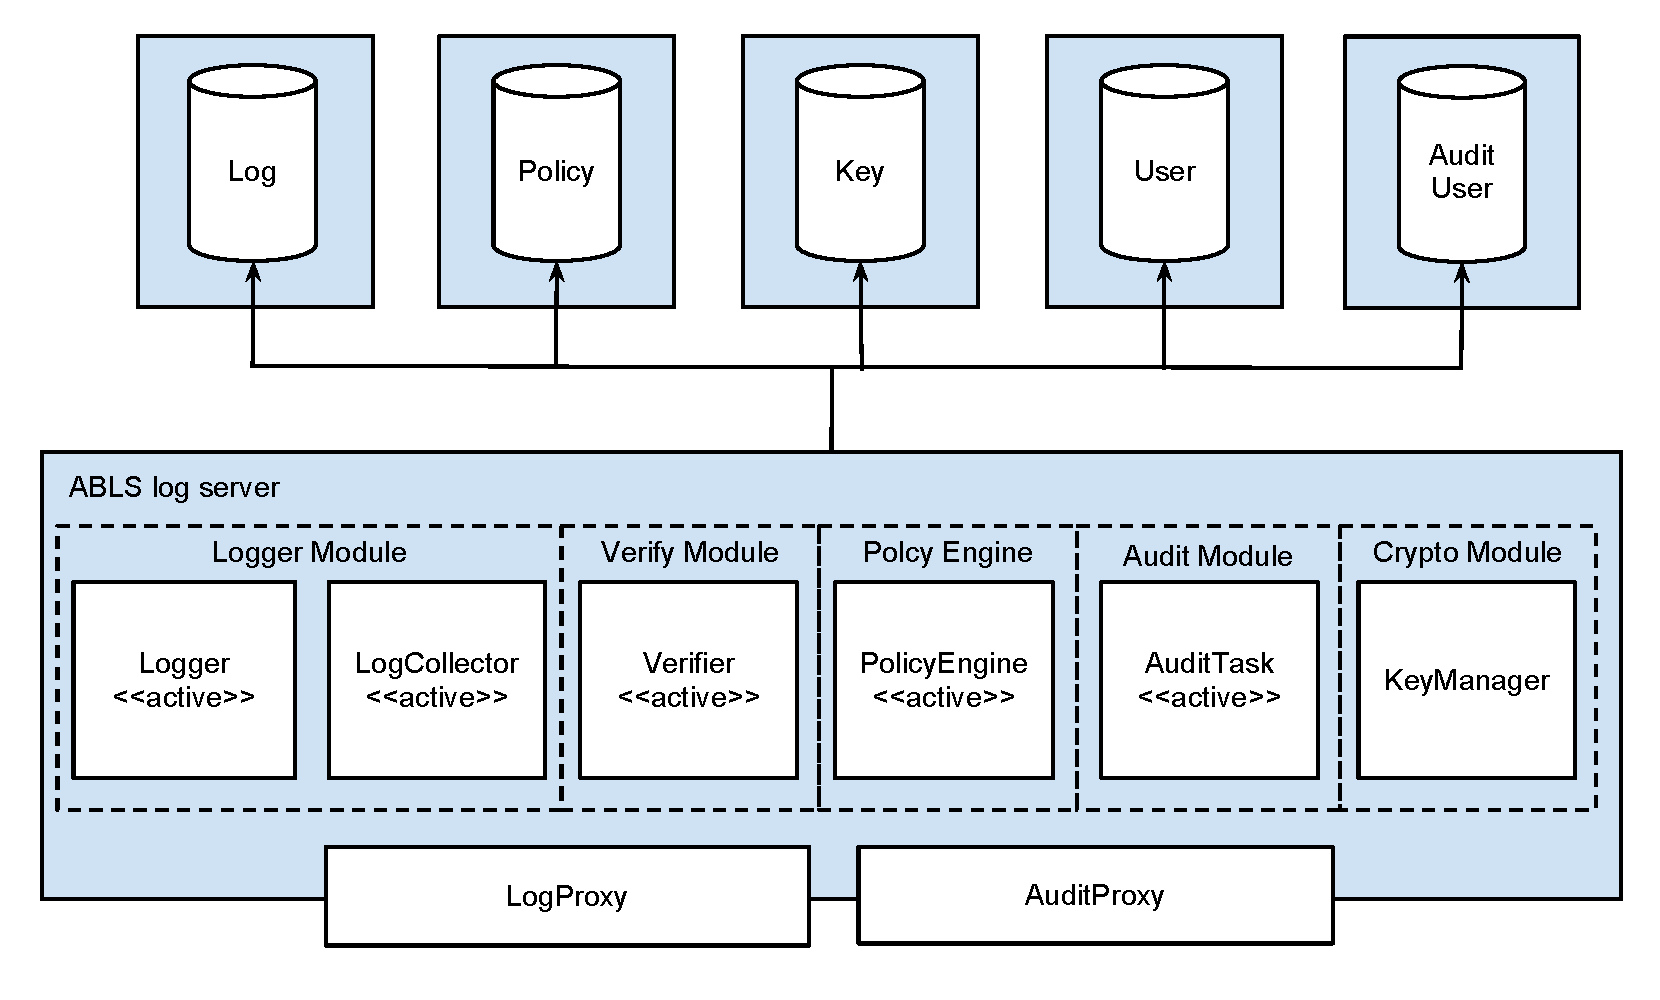
\includegraphics[width=4in]{images/deployment.pdf}
\caption{A high-level depiction of the deployment for an ABLS instance, where each box represents a unique runtime environment (i.e. a unique server).}
\label{fig:deployment}
\end{center}
\end{figure*}

Based on the purpose of each piece of data used in the log, it is best to physically separate databases
that store data of different security classes rather than rely on a single, segregated database that uses MAC with 
polyinstantiation to protect data of different security classes. Of course, access control
and authentication mechanisms for all of the database servers is to be enforced at the operating system level, thus
prohibiting immediate access to all unauthorized users other than the internal tasks (i.e. logger, verifier, policy engine, etc) 
within an ABLS instance. 

In the current ABLS prototype, all database servers are separated as individual SQLite database files. Once
the deployment platform is selected and properly configured, these will be replaced with instances of MySQL 
databases running on separate servers.

\subsection{Hybrid Key Management}
\label{sec:keyMgmt}

Pairing-based cryptography is computationally expensive, and under the assumption that ABLS might be subject 
to very heavy traffic loads at any particular time, the 
overhead of encrypting data to be stored in the database should be as minimal as possible. Therefore, each unique
policy that is needed to encrypt a log message is associated with an AES-256 symmetric key, which is in 
turn encrypted using CP-ABE and then serialized to be stored in the key database. The Charm crypto package allows all cryptographic 
objects (which tend to be nested Python dictionaries and other complicated data structures) to be serialized to byte 
representations for database persistence. This design enhancement enables 
increased throughput without sacrificing the level of confidentiality granularity that is needed for each log entry. 
However, should an unencrypted policy key for a given user's session become compromised, the remaining entries in 
that log database are at risk of being compromised. 

The basic procedure for encrypting a log entry is shown in Algorithm \ref{alg:encrypt}. Once encrypted, the ciphertext
is stored in the database with the rest of the information necessary to continue the log chain for a given user's session.
  
\begin{algorithm}[h] %[htb]
\caption{Log entry encryption} \label{alg:encrypt}
\begin{algorithmic}[1]
\REQUIRE{An unencrypted log entry $L_i$ for session $S_j$ of user $U_k$}
% \ENSURE{The number of all minimum $(s,t)$-cuts of $G$}

% I decided not to list the input/output in this case, so that's why the above two lines are commented out
\STATE{Let $P$ be the access control policy for the message of $L_i$, as determined by the {\tt PolicyEngine}}
\IF{The symmetric key $K$ for $(U_k, S_j)$ has not been generated for $P$}
	\STATE{Generate $K$ and encrypt it with the CP-ABE encryption module using $P$, yielding $K_E$}
	\STATE{Persist $K_E$ to the key database}
\ELSE
	\STATE{Query the database for $K_E$, the encrypted key for policy $P$.}
	\STATE{Decrypt $K_E$ using the attributes of user $U_k$, yielding $K$}
\ENDIF
\STATE{Encrypt $L_i$ with AES-256 using $K$, yielding $E(L_i, K)$}
\STATE{Persist $E(L_i, K)$ to the log database}
\end{algorithmic}
\end{algorithm}

In order to improve the performance of the logger, the per-policy symmetric keys for a user session are kept
in memory until the session has been closed. This avoids the need for the logger to query the database for the key 
when a new log message arrives. 

Also, in order to ensure that every encryption module (cipher) contained within loggers, verifiers, and database 
shims uses the same master key $M_k$, a key manager singleton object was implemented and shared among
all ABLS entities that require the master key. Upon creation, an encryption module will register itself with the key
manager in order to receive any changes made to the master or public key.

\subsection{Database Design}
\label{sec:databaseDesign}

As shown in section \ref{sec:deployment}, there are five main databases that must be maintained by ABLS:
the log, key, user, audit\_user, and policy database. The log database maintains all information in the log chain for every 
single user and session pair. The key database stores the cryptographic keys that were used to construct
such log chains. The user, audit\_user, and policy databases store user information and policy rules for ABLS, respectively. 
In the current prototype of ABLS, the policy database is not used internally. Instead, all event rules are 
hard-coded into the {\tt PolicyEngine}. 

In order to link the entries in the log tables to their corresponding verification and encryption keys in the key database,
common user and session IDs are used (though not as the primary key for the tables since they do not satisfy
the uniqueness property). However, storing user and session information in plaintext may lead to a privacy violation
if the database is compromised. Therefore, using a technique similar to the ``onion encryption'' design in
CryptDB \cite{Popa2012-CryptDB}, this information is now deterministically encrypted before being stored in the database.

This procedure works by encrypting the user and session attributes with a symmetric key generated
from the logger's master key salted by the target table identifier. In mathematical
terms, the encrypted user and session IDs, $[U_i]$ and $[S_j]$, stored in table $T$ are generated as follows.
\begin{align*}
[U_i] = E(M_k || H(T), U_i) \\
[S_j] = E(M_k || H(T), S_j) \\
\end{align*}
In this context, $M_k$ is the master key for the logger. Using the table identifier as a salt to the master key 
enable ensures that tables do not share any common information about the user, which helps prevent against 
inference attacks in the event that the database servers are compromised. Furthermore, this enables verifiers,
who will have access to $M_k$ through the key manager, to decrypt log entries and recover the user identifier 
so that they may check the contents of the other databases as needed.

Also, to better support audits that use the log database, a timestamp field was added to each table as a required
attribute. Not only does such information capture the exact timing of critical system events, it acts as a protection
mechanism in the event that log messages are inserted into the database out of order. Also, it is important to note that
each and every timestamp for a log message is generated when a database entry is generated to be sent to the log 
collector. 

\subsection{Log Querying}
\label{sec:querying}
In order to make ABLS fulfill its purpose as a secure logging system, log query support was added to the audit
module. Such query support is exposed to clients through a lightweight API that is used via the audit protocol.
Currently, only select operations parameterized by the user ID or both the user and session IDs are supported. 
The current version of the API has the following function signatures. \\

\noindent {\tt selectByUser(int uid)} \\
{\tt selectByUserAndSession(int uid, int sid)}\\

To use this API, clients connect to the audit proxy, which is similar to the log traffic proxy, and issue commands according to
the audit protocol to invoke either one of these functions. Once the client is authenticated, they can issue commands to the
audit proxy as JSON strings with the following format. \\

\begin{lstlisting}
{     
    "command" : command_id
    "params" : csv_list
}
\end{lstlisting}

Upon receiving and parsing an incoming command, the client handler, which is spawned to handle each client connection,
issues the appropriate command to the log module to select log message contents from the database. 
A visual depiction of this protocol in action is shown in Figure \ref{fig:protocol}.

\begin{figure}[ht!]
\begin{center}
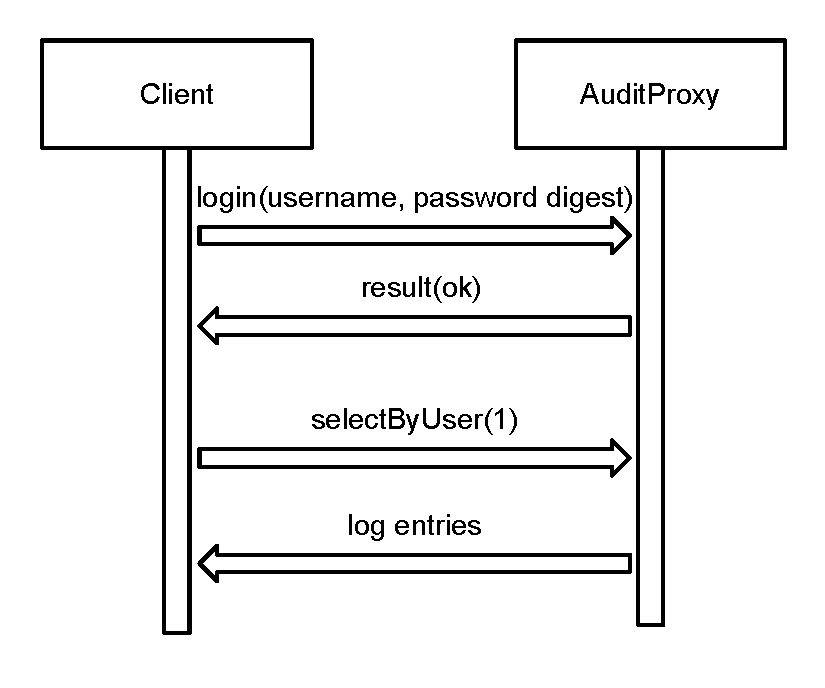
\includegraphics[width=3in]{images/logProtocol.pdf}
\caption{A simplistic sequence diagram of the log protocol, which is highly motivated by the popular FTP protocol.}
\label{fig:protocol}
\end{center}
\end{figure}

Unlike the log proxy, clients for the audit proxy are authenticated using user-defined passwords. Thus, as
part of supporting client authentication, a proper password storage scheme was implemented in which the hash of 
password digests salted by a random string are persisted into the database. In this way, the user password is never sent 
in plaintext over the network. Also, the salt is stored in plaintext in the same audit\_user record, which is a common
design decision for web applications.

\subsection{Log Collection}
As part of the proposed design, all log messages generated by the logger to be inserted into the 
database were to be handed off to a common log collector to do so. This log collector is implemented as a 
separate thread running within the ABLS process and was designed to assume a portion of the database 
communication overhead from loggers to free up cycles for processing more log messages. Each logger instance
points to the same log collector thread. Furthermore, the log collector task is spawned when the ABLS 
instance first loads. Unfortunately, initial performance tests showed that the log collector was consuming too
many CPU cycles from other logger threads, and thus was removed from use in this version of ABLS. 
Future design enhancements may convert the log collector singleton into a log collection service backed 
by a pool of worker threads to handle database activity. 

\subsection{Bootstrapping, Test Enhancement, and Deployment}
In order to streamline the test and deployment phases of development, a bootstrap script was implemented to configure
new (empty) versions of the local SQLite databases. A bootstrap script {\tt Bootstrap.py} was also added to clear the 
contents of every database and insert false user data into the users table. 
The test driver program, {\tt LogProxyDriver.py}, was then modified accordingly to use the default data contained within the 
database. With these changes, the typical process to start and interact with an ABLS instance is as follows.

\begin{enumerate}
	\item Run the bootstrap script to create new versions of the local SQLite databases. In the actual deployment of an ABLS instance, this script would connect to the remote databases and specify their schemas accordingly. Thus, it is meant only for development purposes and should not be used on a live ABLS instance.
	\item Run {\tt Bootstrap.py} to insert fake data into the user database table.
	\item Run the main executable file ({\tt Main.py}) with the -l (log) flag to enable the logging service.	
	\item Run the test driver program ({\tt LogProxyDriver.py}) and point it to the host and port at which the log proxy within the ABLS instance is listening. By default, these are ``localhost'' and port 9998, but they can easily be changed to any other values in the ABLS configuration file. 
\end{enumerate}

Aside from the initialization code, the test driver program includes a robust suite of tests to simulate varying traffic 
loads. The user interface of this program was also improved so as to aid the developers in interacting with the ABLS 
prototype at runtime. Given the difficulty of testing this distributed system at runtime, creating a more sophisticated
test driver was crucial to the development process that enabled smoke tests to be run with minimal effort.

However, despite the complexity of the test driver, it does not, nor will it ever, support the ability to acquire 
diagnostic information from the ABLS runtime. This information is logged by the ABLS instances to the appropriate log 
file, and the administrators for the ABLS system can check this information at their discretion.

\subsection{Log Traffic Encryption}
The ABLS prototype supports SSL encryption of all incoming log traffic to ensure the confidentiality of sensitive
information as it is sent from the client to the server running the log proxy. Unfortunately, this is only one-way SSL 
authentication in which the client verifies the server. Two-way authentication is left for future work, as discussed in
Section \ref{sec:auth}.

\subsection{ABLS Configuration File} 
In order to improve the quality of the ABLS prototype, all of the hard-coded configuration strings that set up databases and 
network settings were removed and placed in a configuration file ({\tt abls.conf}) that is managed by system administrators.
Access to this file can be restricted to system administrators and enforced by the 
operating system. An example of the configuration file is shown below.

\begin{lstlisting}
# Network configuration paramters
abls_host = localhost
abls_logger_port = 9998
abls_audit_port = 9999

# Database configuration string
location.db.log = ~/log.db
location.db.key = ~/key.db
location.db.users = ~/users.db
location.db.audit_users = ~/audit_users.db
location.db.policy = ~/policy.db
\end{lstlisting}

\subsection{Research and Literature Survey}
An initial action item for this work was to investigate the possibility of replacing the relational database model with a 
NoSQL model. I spent a significant amount of time during week 4 investigating the benefits of making a transition
to such a DBMS. In particular, I examined MongoDB, a common document-based NoSQL database. Unfortunately,
my research revealed that MongoDB is not an ACID system, and thus transactions are not guaranteed to keep the
database in a consistent state. In the context of ABLS, a failed transaction could put the system in a bad state. Therefore,
I made the decision to keep the relational database model but hide the user-sensitive information using the techniques
discussed in Section \ref{sec:databaseDesign}.

A comprehensive literature survey on related logging and non-repudiation work was also completed during this phase 
of the project. The corresponding articles that were read are included in this phase's submission package. The digest 
of this work is expected to be a part of the final paper.

\section{ABLS-V2 Design and Implementation}
The final work item for this phase of the project was automated audits of user information according
to audit rules. Unfortunately, given the current log scheme, all context information about a log event is encrypted
and stored in the log message. Even if an audit task was able to decrypt a log payload and 
programmatically determine the details of that particular event, the audit task would need to search over every single
entry in the log database when performing checks against an audit rule. The lack of a unified log format
and audit rule specification made the ultimate task of automating audits infeasible given the current design.
Therefore, I chose to revisit the log generation scheme and corresponding
relational model in an attempt to facilitate more efficient audits. The first step in this process was to define exactly
how audit rules are specified. To this end, I defined a custom audit language LAudit that enables users to specify
audit rules for automated audit tasks. A grammar for the LAudit language is shown below. \\

{\setlength\tabcolsep{4pt}
\begin{tabular}{>{$}l<{$}>{$}r<{$}>{$}l<{$}}
  \text{LRule} &\Coloneqq & \text{USER OPS}\\
  &| & \text{USER OPS OBS} \\
  &| & \text{USER OPS OBS USER} \\
\end{tabular}}

\vspace{.35cm} 
In this context, USER, OPS, and OBS are all finite sets composed of the users, operations, and objects of a
system, as specified by the NIST RBAC model \cite{Sandhu2000-nist-rbac}. While simple, this language effectively
captures the ``who'' and ``what'' of log events. ABLS is capable of appending a timestamp to every that it receives,
which rounds off the log event with ``when'' information. 

ABLS clients must submit log messages according to a pre-defined schema that captures
all of the information in LAudit. The JSON schema used for constructing log messages is shown below.

\begin{lstlisting}
[
    {
        user : int,
        session : int,
        action : int (or String),
        object : int (or String),
        affectedUsers : [int]
    }
]
\end{lstlisting}

In order to capture this information in a relational model to enable efficient queries, a new Event table was added
to the database schema. There is a one-to-one correspondence between Event 
and Log records, and the security of such Event
and Log information is maintained using the same hash chain construction techniques as in the preliminary design.
However, for simplicity, the notion of hash chain epochs was removed.
Also, Action, Object, and AffectedUserGroup tables were added to the database schema to store relevant information
about log events as they are received from the log proxy. A high-level depiction of this new relational model is shown
in Figure \ref{fig:design2}.

\begin{figure}[ht!]
\begin{center}
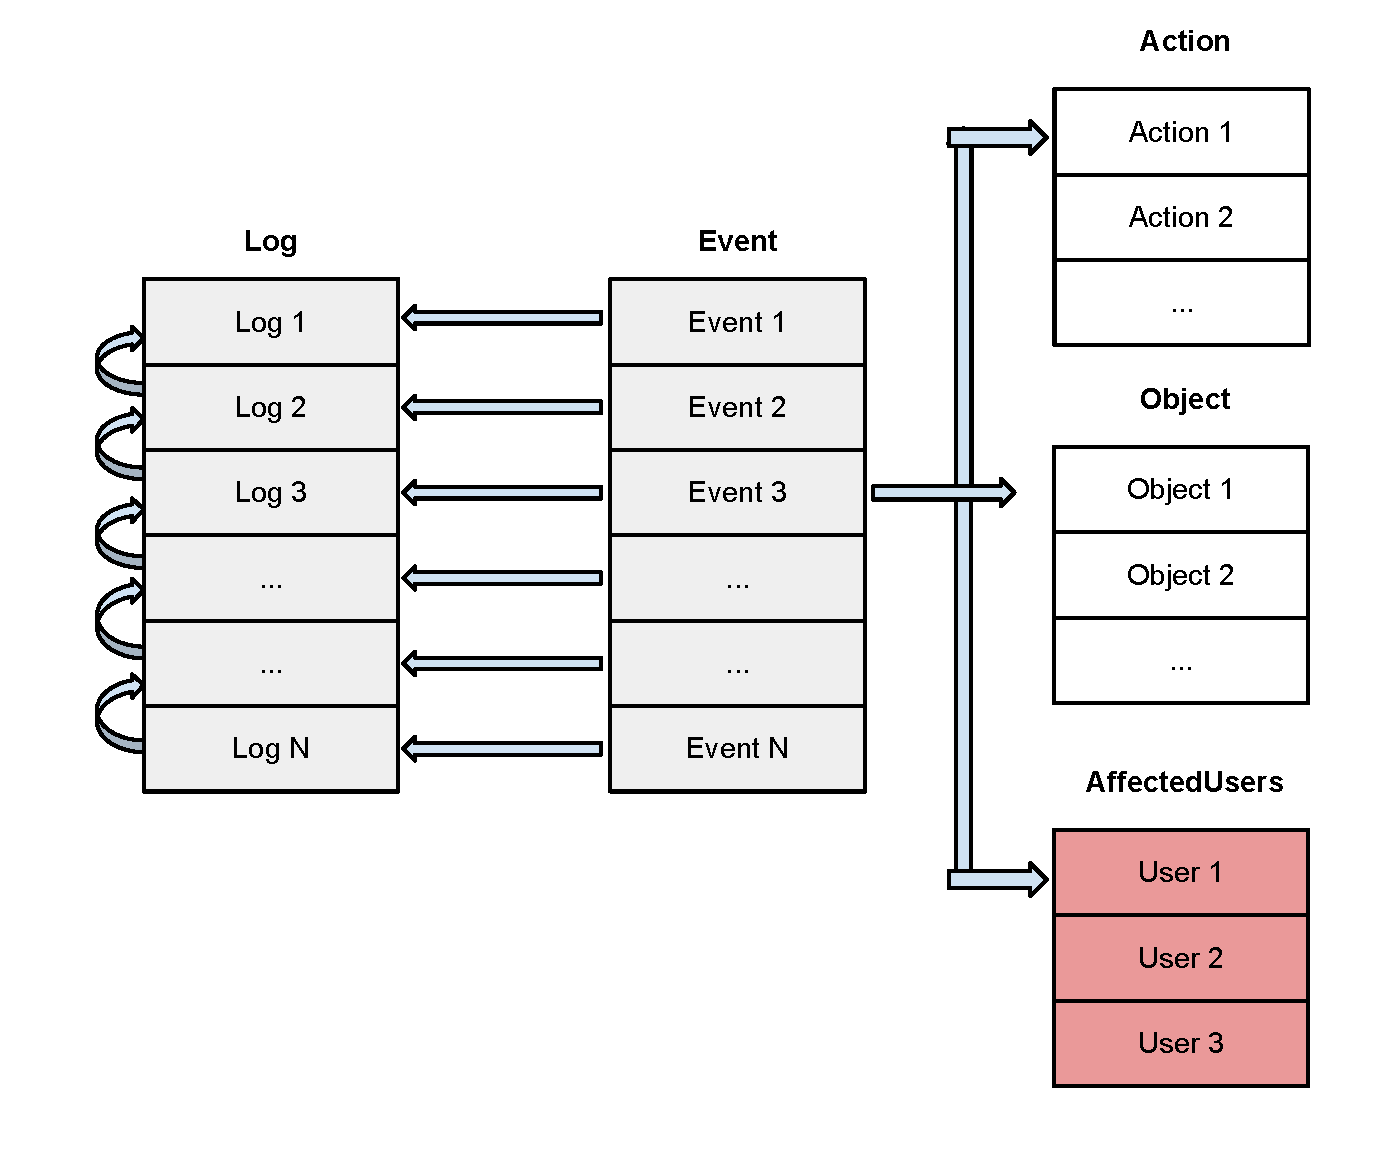
\includegraphics[width=3in]{images/relational_design_v2.pdf}
\caption{A high-level depiction of the new relational data model that supports automated audit tasks.}
\label{fig:design2}
\end{center}
\end{figure}

In this model, all Action and Object records are stored in plaintext. These tables store elements of a finite set, and
encrypting them would not deter a determined attacker. However, all information about affected users is encrypted 
(masked) using the same technique discussed in Section \ref{sec:databaseDesign}. As such, an attacker can infer
information about what types of objects were operated upon, but they cannot determine the specifics of these actions
or the users who performed them without compromising the ABLS master key $M_k$. We feel as though this strikes
a good balance between robust audit specification, reasonable measures of audit and log efficiency, and overall 
log security. 

Audit tasks enforce audit rules using a blacklist approach. Audit rules are specified using the aforementioned 
log message schema and then assigned to audit tasks that periodically run to see if the rules are being properly enforced.
For example, an audit rule might be configured as follows:

\begin{lstlisting}
[
    {
        role : "SuperUser",
        action : "Modified",
        object : "Object-X",
        affectedUsers : [1, 2, 3]
    }
]
\end{lstlisting}

Notice that the user attribute was replaced with a more abstract role attribute. Since it is rare that audit policies will
be specified at the level of individual users, this enables ABLS to enforce more generic audit rules across the 
entire database. If an audit task was given this rule definition, it would query the Event table for all
"Modified" actions performed on objects of type "Object-X" and join the results with the events in the AffectedUserGroup
table. With this data, it would check to see if any of the resulting records have affected users 1, 2, or 3 in them, and if
so, generate an error or alarm. 

The current implementation for ABLS-V2 supports the new log and event chaining, log message parsing, and 
audit task configuration using the aforementioned techniques. However, the code is mostly a proof-of-concept 
implementation, and is not integrated into the entire ABLS system architecture. That is, test-code is embedded
in the {\tt Chainer.py} and {\tt Auditor.py} files to demonstrate that this new automated audit technique works as 
expected.

\section{Postponed Work}
This section contains work items that were omitted from phase 2 due to a lack of time to complete them. However, we include them for completeness since they are essential for future deployments of ABLS.

\subsection{Client Authentication}
\label{sec:auth}
There are two types of clients that can interact with an ABLS instance at runtime: the clients generating log data and the
clients requesting log data for the purpose of auditing. To support log message confidentiality, clients generating 
log data will be authenticated using two-way SSL authentication, as shown in Figure \ref{fig:ssl}. This will 
promote a bidirectional measure of trust between the client and server while at the same time encrypting 
all sensitive data as it is sent between the two endpoints. Also, without an appropriate certificate authority, all
of the certificates will be self-signed for verification purposes. Actual deployments will require these certificates
to be signed by a legitimate CA.

\begin{figure}[ht!]
\begin{center}
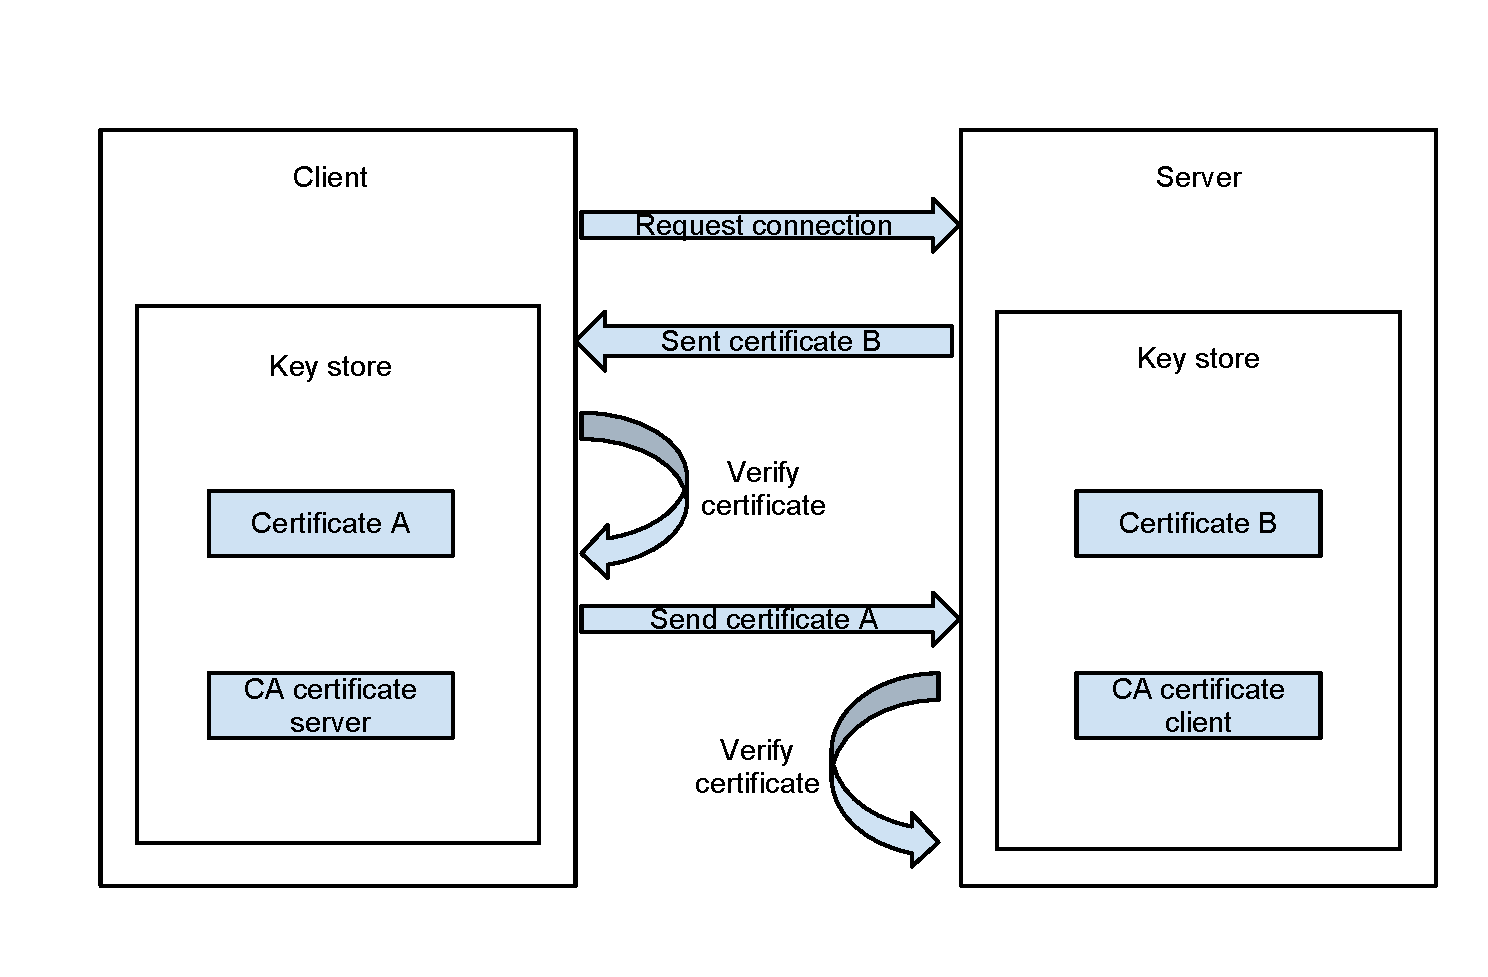
\includegraphics[width=3in]{images/two_way_ssl.pdf}
\caption{A pictorial representation of two-way SSL authentication.}
\label{fig:ssl}
\end{center}
\end{figure}

\section{Attack Strategy}
\label{sec:attack}

My attack strategy for the next phase of the project is two-fold. First, I will use a variety of applicable security-assessment 
tools to automate the detection and exploitation of common vulnerabilities in web applications. 
Specifically, I will use IBM AppScan \cite{_ibm_appscan}, Nessus \cite{_nessus}, and metasploit \cite{_penetration_metasploit} to dynamically test the behavior
of the application once it is deployed. AppScan will serve to automatically scan the application to identify
known vulnerabilities like SQL injection, cross-site scripting, and cross-site request forgeries. Nessus will be used
analyze the network configuration of the application deployment environment. Finally, metasploit, an open-source
alternative to Nessus and AppScan, will be used in the event that neither of these two enterprise products provides
sufficient results in a timely manner. Altogether, these tests will be dynamic in nature and rely on the 
application being deployed at a publicly
accessible server. The goal of these tests is to determine the presence of common vulnerabilities in the web application
and see how they can be used to exploit the backend database. 

In addition to testing the behavior of the application using these tools, I will also conduct a source-code review 
to determine how databases are used, accessed, and modified. In particular, I will examine the implementation of 
authentication code (i.e. password hashing and persistence techniques), user input handling on 
both the client- and server-sides of the environment, and search for hard-coded strings embedded in 
the source code that reveal sensitive information (i.e. database account credentials).

Using the results from these tests, I will then focus intimately on the database using the guidance set forth by 
Ben Natan \cite{ben2005-SDS}. In this part of the ``attack'' phase I make the assumption that I will be given access to the 
server on which the application is deployed, so as to avoid the need to ``hack'' in to conduct a further analysis. 
Depending on the type of DBMS deployed in the application, I will follow the database hardening checklists 
provided by Ben Natan to verify that the databases environments are properly configured. Where possible, I will
use automated tools and configuration scanners to speed up this process.

To finish my analysis I will examine the system configuration and middleware source code with regard to the 
following elements.

\begin{enumerate}
	\item SQL table creation, role definitions, and trigger code.
	\item Database password storage locations and management techniques.
	\item Audit support and configuration.
	\item Data management, caching, and filtering.
\end{enumerate}

This attack strategy will cover network, application, and database vulnerabilities from a configuration
and implementation perspective, and should lead to the production of a solid vulnerability assessment report. 

\begin{comment}
\begin{table}
\centering
\caption{Feelings about Issues}
\begin{tabular}{|l|r|l|} \hline
Flavor&Percentage&Comments\\ \hline
Issue 1 &  10\% & Loved it a lot\\ \hline
Issue 2 &  20\% & Disliked it immensely\\ \hline
Issue 3 &  30\% & Didn't care one bit\\ \hline
Issue 4 &  40\% & Duh?\\ \hline
\end{tabular}
\end{table}

\begin{figure}[ht!]
\label{sample graphic}
\begin{center}
\includegraphics[width=1.5in]{fly.jpg}
\caption{A sample black \& white graphic (JPG).}
\end{center}
\end{figure}
\end{comment}

\bibliographystyle{abbrv}
\bibliography{../../abls}
% You must have a proper ".bib" file
%  and remember to run:
% latex bibtex latex latex
% to resolve all references
\balance
\end{document}
